\documentclass[border=10pt,varwidth]{standalone}

\usepackage{amsmath}

\usepackage{tikz}
\usetikzlibrary{arrows.meta}
\tikzset{%
	>={Latex[width=2mm,length=2mm]},
	% Specifications for style of nodes:
	base/.style = {rectangle, rounded corners, draw=black,
		minimum width=2cm, minimum height=1cm,
		text centered, font=\sffamily, fill=yellow!10},
	var/.style    = {base, fill=blue!20, minimum width=1.2cm, minimum height=0.6cm,},
}

\begin{document}
	\newcommand{\es}{\mathcal{S}}
	\newcommand{\ce}{\boldsymbol{C}}
	\newcommand{\igr}{\boldsymbol{y}}
	\newcommand{\pred}{\boldsymbol{p}}
	Trening
\\
	\begin{minipage}{10cm}
		\begin{center}
			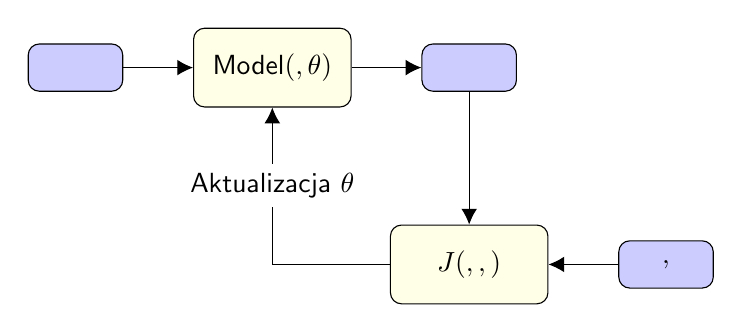
\begin{tikzpicture}[node distance=2.5cm,
			every node/.style={fill=white, font=\sffamily}, align=center]
			\node (x) [var] {$\es$};
			\node (model) [base, right of = x] {Model$(\es, \theta)$};
			\node (y_pred) [var, right of = model] {$\pred$};
			\node (cost) [base, below of = y_pred] {$J(\igr, \pred, \ce)$};
			\node (yp) [var, right of = cost] {$\igr, \ce$};
			
			\draw[->] (x) -- (model);
			\draw[->] (model) -- (y_pred);
			\draw[->] (y_pred) --(cost);
			\draw[->] (cost) -|  node[text width=2.5cm, yshift = 1cm] {Aktualizacja $\theta$} (model);
			\draw[->] (yp) -- (cost);
			\end{tikzpicture}
		\end{center}
	\end{minipage}
\\
\\
	Predykcja
\\
	\begin{minipage}{10cm}
		\begin{center}
			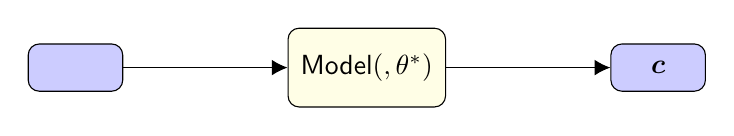
\begin{tikzpicture}[node distance=3.7cm,
			every node/.style={fill=white, font=\sffamily}, align=center]
			\node (x) [var] {$\es$};
			\node (model) [base, right of = x] {Model$(\es, \theta^{*})$};
			\node (y_pred) [var, right of = model] {$\boldsymbol{c}$};
			
			\draw[->] (x) -- (model);
			\draw[->] (model) -- (y_pred);
			\end{tikzpicture}
		\end{center}
	\end{minipage}
\end{document}